\documentclass[notes,11pt, aspectratio=169]{beamer}

\usepackage{pgfpages}
\setbeameroption{hide notes}

\usepackage{helvet}
\usepackage[default]{lato}
\usepackage{array}
\usepackage{tgbonum}

\usepackage{tikz}
\usepackage{verbatim}
\setbeamertemplate{note page}{\pagecolor{yellow!5}\insertnote}
\usetikzlibrary{positioning}
\usetikzlibrary{calc}
\usetikzlibrary{arrows}
\usetikzlibrary{arrows.meta}
\usetikzlibrary{decorations.markings}
\usetikzlibrary{decorations.pathreplacing}
\usetikzlibrary{shapes.misc}
\usetikzlibrary{shapes.geometric}
\usetikzlibrary{matrix,shapes,arrows,fit,tikzmark}
\usepackage{amsmath}
\usepackage{amssymb}
\usepackage{mathtools}
\usepackage{bm}
\usepackage{mathpazo}
\usepackage{hyperref}
%\usepackage{lipsum}
%\usepackage{multimedia}
\usepackage{graphicx}
\usepackage{multirow}
\usepackage{dcolumn}
%\usepackage{bbm}   % PK-only fonts; not renderable by tectonic (indicator uses \mathbf{1})
\usepackage{pgfplots}
\pgfplotsset{compat=1.18}
\usepackage{listings}
\newcolumntype{d}[0]{D{.}{.}{5}}

\usepackage{changepage}
\usepackage{appendixnumberbeamer}
\usepackage[space]{grffile}
\usepackage{booktabs}
\newcommand\independent{\protect\mathpalette{\protect\independenT}{\perp}}
\def\independenT#1#2{\mathrel{\rlap{$#1#2$}\mkern2mu{#1#2}}}
\DeclareMathOperator{\Supp}{Supp}
\DeclareMathOperator*{\argmin}{arg\,min}
\DeclareMathOperator*{\argmax}{arg\,max}
\DeclareMathOperator{\trace}{trace}
\DeclareMathOperator{\softmax}{softmax}
\DeclareMathOperator{\Var}{Var}

\definecolor{blue}{RGB}{0,114,178}
\definecolor{red}{RGB}{213,94,0}
\definecolor{yellow}{RGB}{240,228,66}
\definecolor{green}{RGB}{0,158,115}

\hypersetup{
  colorlinks=true,
  linkbordercolor = {white},
  linkcolor = {blue}
}

\definecolor{MyBackground}{RGB}{255,253,218}

\newenvironment{transitionframe}{
  \setbeamercolor{background canvas}{bg=yellow}
  \begin{frame}}{
    \end{frame}
}

\setbeamercolor{frametitle}{fg=blue}
\setbeamercolor{title}{fg=black}
\setbeamertemplate{footline}[frame number]
\setbeamertemplate{navigation symbols}{}
\setbeamertemplate{itemize items}{-}
\setbeamercolor{itemize item}{fg=blue}
\setbeamercolor{itemize subitem}{fg=blue}
\setbeamercolor{enumerate item}{fg=blue}
\setbeamercolor{enumerate subitem}{fg=blue}
\setbeamercolor{button}{bg=MyBackground,fg=blue,}

\setbeamercolor{section in toc}{fg=blue}
\setbeamercolor{subsection in toc}{fg=red}
\setbeamersize{text margin left=1em,text margin right=1em}

\newenvironment{wideitemize}{\itemize\addtolength{\itemsep}{10pt}}{\enditemize}

\lstset{
    language=Python,
    basicstyle=\ttfamily\scriptsize,
    keywordstyle=\color{blue}\bfseries,
    stringstyle=\color{red!70!black},
    commentstyle=\color{green!50!black}\itshape,
    numbers=left,
    numberstyle=\tiny\color{gray},
    numbersep=5pt,
    frame=single,
    breaklines=true,
    backgroundcolor=\color{gray!5},
    showstringspaces=false,
    tabsize=4
}

\newcommand{\va}{\mathbf{a}}
\newcommand{\vb}{\mathbf{b}}
\newcommand{\vc}{\mathbf{c}}
\newcommand{\vh}{\mathbf{h}}
\newcommand{\vk}{\mathbf{k}}
\newcommand{\vo}{\mathbf{o}}
\newcommand{\vq}{\mathbf{q}}
\newcommand{\vs}{\mathbf{s}}
\newcommand{\vu}{\mathbf{u}}
\newcommand{\vv}{\mathbf{v}}
\newcommand{\vw}{\mathbf{w}}
\newcommand{\vx}{\mathbf{x}}
\newcommand{\vy}{\mathbf{y}}
\newcommand{\vz}{\mathbf{z}}
\newcommand{\vK}{\mathbf{K}}
\newcommand{\vQ}{\mathbf{Q}}
\newcommand{\vV}{\mathbf{V}}
\newcommand{\vW}{\mathbf{W}}
\newcommand{\vX}{\mathbf{X}}
\newcommand{\vY}{\mathbf{Y}}
\newcommand{\vO}{\mathbf{O}}
\newcommand{\R}{\mathbb{R}}
\newcommand{\E}{\mathbb{E}}


\title[]{\textcolor{blue}{Machine Learning II}\\ \textcolor{black}{\normalsize Lecture 6: Attention and Self-Attention}}
\author[Quispe]{}
\institute[ENEI]{\small{Alexander Quispe \\ ENEI -- INEI \,\textperiodcentered\, PEU-CD 2026}}
\date{October 23, 2026}


\begin{document}

\begin{frame}[plain]\titlepage\end{frame}

\begin{frame}{Outline}\tableofcontents\end{frame}


\tikzset{
        every picture/.style={remember picture,baseline},
        every node/.style={anchor=base,align=center,outer sep=1.5pt},
        every path/.style={thick},
        }
\tikzstyle{every picture}+=[remember picture]
\tikzstyle{mybox} =[draw=black, very thick, rectangle, inner sep=10pt, inner ysep=20pt]
\tikzstyle{fancytitle} =[draw=black,fill=red, text=white]




% ============================================================
\section{Recap and Motivation}
% ============================================================

\begin{transitionframe}
\begin{center}
{\Huge \textbf{Recap \& Motivation}}\\[10pt]
{\large The bottleneck of seq2seq}
\end{center}
\end{transitionframe}

\begin{frame}
\frametitle{Where We Left Off}

\textbf{Lectures so far:}
\begin{itemize}
    \item L1--L3: MLP, backprop, regularization.
    \item L4: CNNs for spatial data.
    \item L5: RNN, LSTM, GRU for sequential data.
    \item L6--L7: latent factor models, embeddings (lookup and learned).
\end{itemize}

\vspace{8pt}
\textbf{Key idea from L7:} embed each token into a vector. A sentence becomes a sequence of vectors.

\vspace{8pt}
\textbf{Today's question:} when a model processes a sequence, how should each position decide \emph{which other positions to look at}?

\vspace{6pt}
\textcolor{red}{Attention is the answer. It started as a fix for RNN seq2seq, then took over deep learning.}
\end{frame}

\begin{frame}
\frametitle{Mini-Recap: What Is an Encoder?}

\textbf{Encoder = read the input sequence and build hidden states.}

\vspace{6pt}
\begin{center}
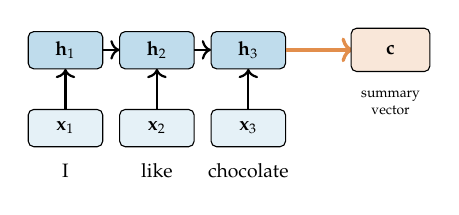
\begin{tikzpicture}[scale=0.86, every node/.style={font=\scriptsize}]
    \foreach \i/\w in {1/I, 2/like, 3/chocolate} {
        \draw[fill=blue!10, rounded corners=2pt] (\i*1.35-1.35, 0) rectangle (\i*1.35-0.25, 0.55);
        \node at (\i*1.35-0.8, 0.28) {$\vx_\i$};
        \node at (\i*1.35-0.8, -0.35) {\w};
    }
    \foreach \i in {1,2,3} {
        \draw[fill=blue!25, rounded corners=2pt] (\i*1.35-1.35, 1.15) rectangle (\i*1.35-0.25, 1.7);
        \node at (\i*1.35-0.8, 1.43) {$\vh_\i$};
        \draw[->, thick] (\i*1.35-0.8, 0.55) -- (\i*1.35-0.8, 1.15);
    }
    \foreach \i in {1,2} {
        \pgfmathsetmacro\x{\i*1.35-0.25}
        \pgfmathsetmacro\nx{\i*1.35}
        \draw[->, thick] (\x, 1.43) -- (\nx, 1.43);
    }
    \draw[->, very thick, red!70] (3.8, 1.43) -- (4.8, 1.43);
    \node[draw, fill=red!15, rounded corners=2pt, minimum width=1cm, minimum height=0.55cm] at (5.35, 1.43) {$\vc$};
    \node[font=\tiny, align=center] at (5.35, 0.65) {summary\\vector};
\end{tikzpicture}
\end{center}

\vspace{4pt}
\[
    \vh_t = f(\vx_t, \vh_{t-1}; \mathbf{w}_e),
    \qquad
    \vc = \vh_T.
\]

\textcolor{blue}{The encoder does not translate yet. It turns the source sentence into a sequence of memories, ending with a summary.}
\end{frame}

\begin{frame}
\frametitle{Mini-Recap: What Is a Decoder?}

\textbf{Decoder = generate the output sequence one token at a time.}

\vspace{6pt}
\begin{center}
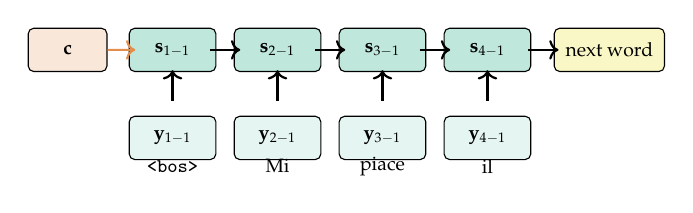
\begin{tikzpicture}[scale=0.86, every node/.style={font=\scriptsize}]
    \node[draw, fill=red!15, rounded corners=2pt, minimum width=1cm, minimum height=0.55cm] (c) at (0, 1.3) {$\vc$};
    \foreach \i/\w in {1/\texttt{<bos>}, 2/Mi, 3/piace, 4/il} {
        \pgfmathsetmacro\x{\i*1.55}
        \node[draw, fill=green!10, rounded corners=2pt, minimum width=1.1cm, minimum height=0.55cm] at (\x, 0) {$\vy_{\i-1}$};
        \node at (\x, -0.42) {\w};
        \node[draw, fill=green!25, rounded corners=2pt, minimum width=1.1cm, minimum height=0.55cm] at (\x, 1.3) {$\vs_{\i-1}$};
        \draw[->, thick] (\x, 0.55) -- (\x, 1.0);
    }
    \foreach \i in {1,2,3} {
        \pgfmathsetmacro\x{\i*1.55+0.55}
        \pgfmathsetmacro\nx{\i*1.55+1.0}
        \draw[->, thick] (\x, 1.3) -- (\nx, 1.3);
    }
    \draw[->, red!70, thick] (c) -- (1.0, 1.3);
    \node[draw, fill=yellow!30, rounded corners=2pt, minimum width=1.4cm, minimum height=0.55cm] at (8.0, 1.3) {next word};
    \draw[->, thick] (6.8, 1.3) -- (7.25, 1.3);
\end{tikzpicture}
\end{center}

\vspace{4pt}
\[
    \vs_t = g(\vy_{t-1}, \vs_{t-1}, \vc; \mathbf{w}_d),
    \qquad
    p(\vy_t \mid \vy_{<t}, \vx_{1:T}) = \softmax(W_o \vs_t).
\]

\textcolor{blue}{The decoder is a conditional language model: it writes the target sentence while conditioned on $\vc$.}
\end{frame}

\begin{frame}
\frametitle{Numerical Mini-Example: Decoder Softmax}

\textbf{Suppose the decoder must choose the next Italian word after ``Mi piace il''.}

\vspace{4pt}
\begin{center}
\renewcommand{\arraystretch}{1.15}
\small
\begin{tabular}{l c c c}
\toprule
\textbf{candidate word} & cioccolato & cane & perché \\
\midrule
\textbf{logit} $z_i$ & 2.0 & 1.0 & 0.0 \\
\textbf{$\exp(z_i)$} & 7.39 & 2.72 & 1.00 \\
\textbf{probability} & 0.67 & 0.24 & 0.09 \\
\bottomrule
\end{tabular}
\end{center}

\vspace{6pt}
\[
    \softmax(2,1,0)
    =
    \frac{(e^2,e^1,e^0)}{e^2+e^1+e^0}
    \approx
    (0.67, 0.24, 0.09).
\]

\textcolor{red}{Interpretation:} the decoder is not directly outputting a word; it outputs a probability distribution over the vocabulary.
\end{frame}

\begin{frame}
\frametitle{RNN Seq2Seq Recap}

\textbf{Seq2seq idea:} encode the source sentence into one vector, then decode the target sentence from it
(Sutskever et al.\ 2014, Cho et al.\ 2014).

\vspace{6pt}
\begin{center}
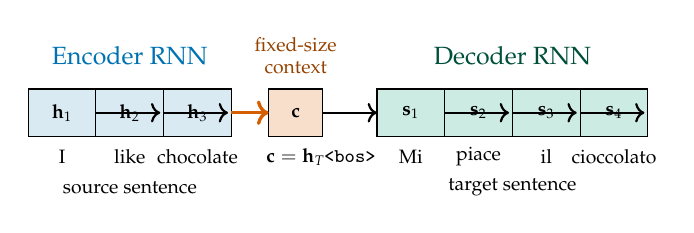
\begin{tikzpicture}[scale=0.86, every node/.style={font=\scriptsize}]
    \foreach \i/\w in {1/I, 2/like, 3/chocolate} {
        \draw[fill=blue!15] (\i-1, 0) rectangle (\i, 0.7);
        \node at (\i-0.5, 0.35) {$\vh_\i$};
        \node at (\i-0.5, -0.3) {\w};
    }
    \foreach \i in {1,2} {
        \pgfmathtruncatemacro\next{\i+1}
        \draw[->, thick] (\i, 0.35) -- (\next-0.05, 0.35);
    }

    \node[font=\small, blue] at (1.5, 1.2) {Encoder RNN};
    \node at (1.5, -0.75) {source sentence};

    \draw[fill=red!20] (3.55, 0) rectangle (4.35, 0.7);
    \node at (3.95, 0.35) {$\vc$};
    \node at (3.95, -0.3) {$\vc = \vh_T$};
    \draw[->, very thick, red] (3, 0.35) -- (3.55, 0.35);
    \node[font=\scriptsize, red!70!black, align=center] at (3.95, 1.2) {fixed-size\\context};

    \node at (4.75, -0.3) {\texttt{<bos>}};
    \draw[->, thick] (4.35, 0.35) -- (5.15, 0.35);

    \foreach \i/\w in {1/Mi, 2/piace, 3/il, 4/cioccolato} {
        \pgfmathsetmacro\x{\i+5.15}
        \draw[fill=green!20] (\x-1, 0) rectangle (\x, 0.7);
        \node at (\x-0.5, 0.35) {$\vs_\i$};
        \node at (\x-0.5, -0.3) {\w};
    }
    \foreach \i in {1,2,3} {
        \pgfmathsetmacro\x{\i+5.15}
        \pgfmathsetmacro\nx{\x+1}
        \draw[->, thick] (\x, 0.35) -- (\nx-0.05, 0.35);
    }

    \node[font=\small, green!50!black] at (7.15, 1.2) {Decoder RNN};
    \node at (7.15, -0.75) {target sentence};
\end{tikzpicture}
\end{center}

\vspace{6pt}
\textbf{Equations:}
\small
\begin{align*}
    \vh_t &= f(\vx_t, \vh_{t-1}; \mathbf{w}_e) \quad &&\text{encode} \\
    \vc &= \vh_T \quad &&\text{fixed context vector} \\
    \vs_t &= g(\vy_{t-1}, \vs_{t-1}, \vc; \mathbf{w}_d) \quad &&\text{decode}
\end{align*}
\normalsize

\textbf{Limitation:} all source information must pass through one vector $\vc$.
This works for short sentences, but becomes a bottleneck.
\end{frame}

\begin{frame}
\frametitle{The Bottleneck Problem}

\textbf{Empirical observation} (Bahdanau, Cho, Bengio 2014): translation quality \emph{drops sharply} for long source sentences.

\vspace{3pt}
\begin{center}
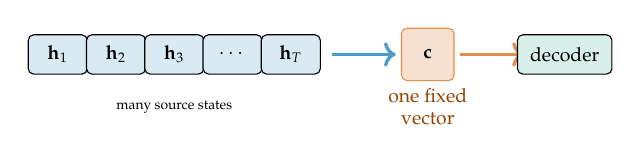
\begin{tikzpicture}[scale=0.74, every node/.style={font=\scriptsize}]
    \foreach \i/\lab in {0/$\vh_1$, 1/$\vh_2$, 2/$\vh_3$, 3/$\cdots$, 4/$\vh_T$} {
        \node[draw, fill=blue!15, rounded corners=2pt, minimum width=0.75cm, minimum height=0.5cm] at (\i*1.0, 0) {\lab};
    }
    \draw[->, very thick, blue!70] (4.7, 0) -- (5.8, 0);
    \draw[fill=red!18, draw=red!70, rounded corners=2pt] (5.9, -0.45) rectangle (6.8, 0.45);
    \node at (6.35, 0) {$\vc$};
    \node[align=center, red!70!black] at (6.35, -0.9) {one fixed\\vector};
    \draw[->, very thick, red!70] (6.9, 0) -- (8.0, 0);
    \node[draw, fill=green!15, rounded corners=2pt, minimum width=1.2cm, minimum height=0.5cm] at (8.7, 0) {decoder};
    \node[align=center, font=\tiny] at (2.0, -0.9) {many source states};
\end{tikzpicture}
\end{center}

\vspace{2pt}
\textbf{The information bottleneck:}
a fixed-dim vector $\vc \in \R^d$ must summarize the whole source sentence.

\vspace{4pt}
\textbf{Why this is hard for RNNs to fix on their own:}
\begin{itemize}
    \item Information from $\vx_1$ has to flow through $\vh_2, \vh_3, \ldots, \vh_T$ before reaching $\vc$.
    \item Word-by-word alignment between source and target is not captured.
\end{itemize}

\vspace{3pt}
\textcolor{red}{Idea (Bahdanau et al.\ 2014):} let the decoder \emph{look back} at the encoder hidden states $\vh_1, \ldots, \vh_T$ -- not just the final $\vc$.
\end{frame}

\begin{frame}
\frametitle{Today's Roadmap (Annotated)}

\begin{enumerate}
    \item \textbf{Bahdanau attention.} Derive attention as a fix for the seq2seq bottleneck.
    \item \textbf{Query-Key-Value.} The abstraction that generalizes attention.
    \item \textbf{Self-attention.} What if Q, K, V all come from the same sequence?
    \item \textbf{Why $\sqrt{d_k}$?} The math behind scaled dot-product attention (CLT derivation -- needed for HW3).
    \item \textbf{Multi-head attention.} Many attention computations in parallel.
    \item \textbf{Practical implementation.} PyTorch, masking, batch dims.
    \item \textbf{Bridge to Transformers.} What's missing for Lecture 9.
\end{enumerate}
\end{frame}


% ============================================================
\section{Bahdanau Attention}
% ============================================================

\begin{transitionframe}
\begin{center}
{\Huge \textbf{Bahdanau Attention}}\\[10pt]
{\large Three ideas, one mechanism}
\end{center}
\end{transitionframe}

\begin{frame}
\frametitle{Idea 1: Symmetrize Input and Output}

\textbf{Old seq2seq:} decoder uses only the final encoder state $\vc$.

\vspace{8pt}
\textbf{New idea:} decoder uses \emph{all} encoder states $\vh_1, \ldots, \vh_T$.

\vspace{6pt}
\begin{center}
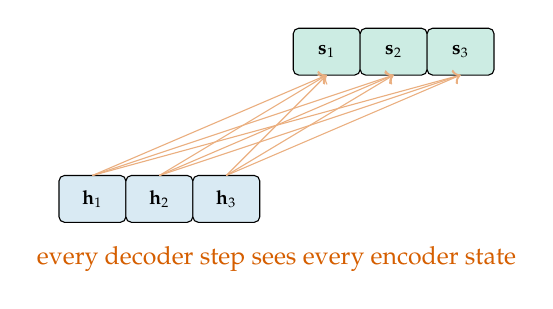
\begin{tikzpicture}[scale=0.85, every node/.style={font=\scriptsize}]
    \foreach \i in {1,...,3} {
        \draw[fill=blue!15, rounded corners=2pt] (\i-1, 0) rectangle (\i, 0.7);
        \node at (\i-0.5, 0.35) {$\vh_\i$};
    }
    \foreach \i in {1,...,3} {
        \pgfmathsetmacro\x{\i+3.5}
        \draw[fill=green!20, rounded corners=2pt] (\x-1, 2.2) rectangle (\x, 2.9);
        \node at (\x-0.5, 2.55) {$\vs_\i$};
    }

    \foreach \i in {1,...,3} {
        \foreach \j in {1,...,3} {
            \pgfmathsetmacro\sx{\i-0.5}
            \pgfmathsetmacro\dx{\j+3}
            \draw[->, red!50, thin] (\sx, 0.7) -- (\dx, 2.2);
        }
    }
    \node[font=\small, red] at (3.25, -0.55) {every decoder step sees every encoder state};
\end{tikzpicture}
\end{center}

\vspace{8pt}
\textbf{Simplest version:} the new context is just the average of encoder states:
\[
    \vc \;=\; \frac{1}{T}\sum_{\tau=1}^T \vh_\tau.
\]

\textcolor{red}{But this loses positional information.} Each output position uses the same average. Bad.
\end{frame}

\begin{frame}
\frametitle{Idea 2: Make Context Specific to Each Output}

\textbf{Improvement:} let each decoder step $t$ compute its \emph{own} weighted average over encoder states.

\vspace{6pt}
\textbf{Per-output context:}
\[
    \vc_t \;=\; \sum_{\tau=1}^T \alpha_{t,\tau}\, \vh_\tau.
\]

\vspace{4pt}
where $\alpha_{t,\tau} \in \R$ tells us how much output position $t$ should attend to input position $\tau$.

\vspace{8pt}
\textbf{Question:} how do we set $\alpha_{t,\tau}$?

\vspace{4pt}
\textbf{Answer:} learn it from the data, as a similarity between the decoder state $\vs_{t-1}$ and the encoder state $\vh_\tau$.

\vspace{8pt}
\textbf{Simplest similarity: dot product.}
\[
    e_{t,\tau} \;=\; \langle \vs_{t-1}, \vh_\tau \rangle.
\]

\textcolor{red}{Still missing:} the $e_{t,\tau}$ are raw scores, not probabilities. They can be negative, unbounded, hard to interpret.
\end{frame}

\begin{frame}
\frametitle{Idea 3: Normalize via Softmax}

\textbf{Convert scores to probabilities} using softmax over the input positions:
\[
    \alpha_{t,\tau} \;=\; \frac{\exp(e_{t,\tau})}{\sum_{\tau'=1}^T \exp(e_{t,\tau'})}.
\]

\vspace{4pt}
Now $\alpha_{t,\tau} \geq 0$ and $\sum_\tau \alpha_{t,\tau} = 1$.

\vspace{5pt}
\begin{center}
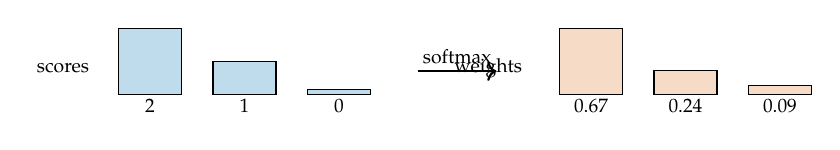
\begin{tikzpicture}[x=1cm, y=0.42cm, every node/.style={font=\scriptsize}]
    \node[anchor=east] at (-0.25, 3.2) {scores};
    \foreach \i/\s/\h in {0/2/2.0, 1/1/1.0, 2/0/0.15} {
        \draw[fill=blue!25] (\i*1.2, 2.4) rectangle (\i*1.2+0.8, 2.4+\h);
        \node at (\i*1.2+0.4, 2.05) {$\s$};
    }
    \draw[->, thick] (3.8, 3.1) -- (4.8, 3.1);
    \node at (4.3, 3.55) {softmax};
    \node[anchor=east] at (5.25, 3.2) {weights};
    \foreach \i/\s/\h in {0/0.67/2.0, 1/0.24/0.72, 2/0.09/0.27} {
        \draw[fill=red!22] (5.6+\i*1.2, 2.4) rectangle (5.6+\i*1.2+0.8, 2.4+\h);
        \node at (6.0+\i*1.2, 2.05) {$\s$};
    }
\end{tikzpicture}
\end{center}

\vspace{3pt}
\textcolor{red}{Softmax turns raw scores into an alignment distribution.}
\end{frame}

\begin{frame}
\frametitle{Bahdanau Attention Recipe}

\textbf{At each decoder step $t$, repeat the same three operations:}

\vspace{2pt}
\small
\begin{align*}
    \text{score:} \quad
    e_{t,\tau} &= \langle \vs_{t-1}, \vh_\tau \rangle
    &\quad
    \text{normalize:} \quad
    \alpha_{t,\tau} &= \softmax_\tau(e_{t,\tau}) \\
    \text{average:} \quad
    \vc_t &= \sum_\tau \alpha_{t,\tau}\, \vh_\tau
\end{align*}
\normalsize

\vspace{-3pt}
\begin{center}
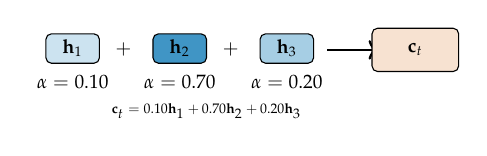
\begin{tikzpicture}[scale=0.68, every node/.style={font=\scriptsize}]
    \foreach \x/\lab/\a/\op in {0/$\vh_1$/0.10/20, 2/$\vh_2$/0.70/75, 4/$\vh_3$/0.20/35} {
        \draw[fill=blue!\op, rounded corners=2pt] (\x, 0) rectangle (\x+1.0, 0.55);
        \node at (\x+0.5, 0.28) {\lab};
        \node at (\x+0.5, -0.35) {$\alpha=\a$};
    }
    \node at (1.45, 0.25) {$+$};
    \node at (3.45, 0.25) {$+$};
    \draw[->, thick] (5.25, 0.25) -- (6.2, 0.25);
    \node[draw, fill=red!18, rounded corners=2pt, minimum width=1.1cm, minimum height=0.55cm] at (6.9, 0.25) {$\vc_t$};
    \node[font=\tiny] at (3.0, -0.9) {$\vc_t = 0.10\vh_1 + 0.70\vh_2 + 0.20\vh_3$};
\end{tikzpicture}
\end{center}

\vspace{-2pt}
\textbf{Then decode using this context:} $\vs_t = g(\vy_{t-1}, \vs_{t-1}, \vc_t; \mathbf{w}_d)$.

\vspace{3pt}
\textcolor{blue}{Next: rename this pattern as query, key, value.}
\end{frame}

\begin{frame}
\frametitle{Numerical Mini-Example: Weighted Context}

\textbf{Suppose the decoder puts most attention on the second source word.}

\vspace{4pt}
\[
    \vh_1 =
    \begin{bmatrix} 1 \\ 0 \end{bmatrix},
    \qquad
    \vh_2 =
    \begin{bmatrix} 0 \\ 2 \end{bmatrix},
    \qquad
    \vh_3 =
    \begin{bmatrix} 2 \\ 1 \end{bmatrix},
    \qquad
    \alpha = (0.10, 0.70, 0.20).
\]

\vspace{2pt}
\begin{align*}
    \vc_t
    &= 0.10\vh_1 + 0.70\vh_2 + 0.20\vh_3 \\
    &= 0.10
    \begin{bmatrix} 1 \\ 0 \end{bmatrix}
    + 0.70
    \begin{bmatrix} 0 \\ 2 \end{bmatrix}
    + 0.20
    \begin{bmatrix} 2 \\ 1 \end{bmatrix} \\
    &=
    \begin{bmatrix} 0.10 \\ 0 \end{bmatrix}
    +
    \begin{bmatrix} 0 \\ 1.40 \end{bmatrix}
    +
    \begin{bmatrix} 0.40 \\ 0.20 \end{bmatrix}
    =
    \begin{bmatrix} 0.50 \\ 1.60 \end{bmatrix}.
\end{align*}

\textcolor{red}{Interpretation:} attention builds a new vector by mixing source states, not by choosing only one.
\end{frame}

\begin{frame}
\frametitle{Worked Example: ``Boys' Age?''}

\textbf{Setup} (from Caltech CS148): we have five people.

\vspace{2pt}
\begin{center}
\renewcommand{\arraystretch}{1.1}
\scriptsize
\begin{tabular}{l c c c c c}
\toprule
Name (\textbf{key}) & Joseph & Wendy & Nellie & Mary & Theodore \\
\midrule
Boy? (1=yes) & 1 & 0 & 0 & 0 & 1 \\
Age (\textbf{value}) & 11 & 5 & 8 & 3 & 7 \\
\bottomrule
\end{tabular}
\end{center}

\vspace{5pt}
\textbf{Query:} ``what is the average age of the \emph{boys}?''

\vspace{2pt}
The query says ``look at boys''. The keys say who is a boy. The values are the ages.

\vspace{5pt}
\textbf{Compute weights} (hard-attention intuition: keep boys, mask others):
\[
    \alpha = (\,0.5,\; 0,\; 0,\; 0,\; 0.5\,) \quad \text{after masking + normalization}.
\]

\textbf{Weighted sum of values:}
\[
    0.5 \cdot 11 \;+\; 0 \cdot 5 \;+\; 0 \cdot 8 \;+\; 0 \cdot 3 \;+\; 0.5 \cdot 7 \;=\; 9.
\]

\textcolor{red}{Query asks, keys match, values are averaged.}
\end{frame}

\begin{frame}
\frametitle{Visual: Bahdanau Attention Heatmap}

\textbf{Real attention} (Bahdanau et al.\ 2014, En-Fr):

\begin{columns}[T]
\begin{column}{0.5\textwidth}
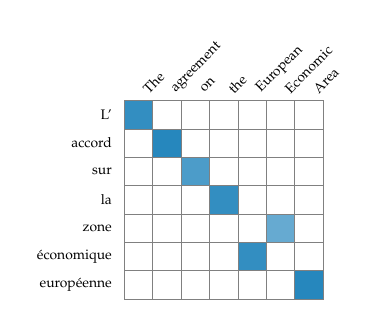
\begin{tikzpicture}[scale=0.36, every node/.style={font=\tiny}]
    \foreach \i/\w in {0/The, 1/agreement, 2/on, 3/the, 4/European, 5/Economic, 6/Area} {
        \node[rotate=45, anchor=west] at (\i+0.5, 0.1) {\w};
    }
    \foreach \j/\w in {0/L', 1/accord, 2/sur, 3/la, 4/zone, 5/\'{e}conomique, 6/europ\'{e}enne} {
        \node[anchor=east] at (-0.1, -\j-0.5) {\w};
    }

    \foreach \i/\j/\v in {0/0/0.8, 1/1/0.85, 2/2/0.7, 3/3/0.8, 4/5/0.8, 5/4/0.6, 6/6/0.85} {
        \fill[blue, opacity=\v] (\i, -\j-1) rectangle (\i+1, -\j);
    }
    \foreach \i in {0,...,6} {
        \foreach \j in {0,...,6} {
            \draw[gray, very thin] (\i, -\j) rectangle (\i+1, -\j-1);
        }
    }
\end{tikzpicture}
\end{column}
\begin{column}{0.5\textwidth}
\vspace{1cm}
\textbf{Reading the heatmap:}

\vspace{4pt}
Bright cells = high $\alpha_{t,\tau}$.

\vspace{4pt}
The diagonal pattern shows mostly-monotonic alignment, with \emph{local reordering}:

\vspace{2pt}
\hspace{6pt}``European Economic Area''

\hspace{6pt}$\;\;\leftrightarrow$ ``zone \'{e}conomique europ\'{e}enne''.

\vspace{6pt}
\textcolor{blue}{No alignment supervision -- it emerges from end-to-end training.}
\end{column}
\end{columns}
\end{frame}

\begin{frame}
\frametitle{Section Summary}

\textbf{What changed relative to old seq2seq?}

\vspace{6pt}
\begin{itemize}
    \item Old decoder: every output uses the same fixed vector $\vc = \vh_T$.
    \item Attention decoder: each output gets its own context $\vc_t$.
    \item The weights $\alpha_{t,\tau}$ act like a soft alignment between target position $t$ and source position $\tau$.
\end{itemize}

\vspace{8pt}
\begin{tikzpicture}
\node [mybox] (box){%
    \begin{minipage}{0.9\textwidth}
    \centering
    decoder state $\vs_{t-1}$ asks a question; encoder states $\vh_\tau$ answer it.
    \end{minipage}
};
\end{tikzpicture}

\vspace{6pt}
\textcolor{red}{Coming up:} rename these roles as query, key, and value.
\end{frame}


% ============================================================
\section{Query, Key, Value}
% ============================================================

\begin{transitionframe}
\begin{center}
{\Huge \textbf{Query, Key, Value}}\\[10pt]
{\large The general abstraction}
\end{center}
\end{transitionframe}

\begin{frame}
\frametitle{Three Roles in Attention}

\textbf{Reread Bahdanau attention with new names:}

\vspace{4pt}
\begin{center}
\renewcommand{\arraystretch}{1.15}
\scriptsize
\begin{tabular}{l l l}
\toprule
\textbf{Role} & \textbf{Bahdanau} & \textbf{What it does} \\
\midrule
\textbf{Query} $\vq$ & $\vs_{t-1}$ (decoder state) & ``what am I looking for?'' \\
\textbf{Key} $\vk_\tau$ & $\vh_\tau$ (encoder state) & ``what do I represent for matching?'' \\
\textbf{Value} $\vv_\tau$ & $\vh_\tau$ (encoder state) & ``what do I contribute if matched?'' \\
\bottomrule
\end{tabular}
\end{center}

\vspace{5pt}
\textbf{Same recipe, now in Q/K/V language:}
\small
\begin{align*}
    e_\tau &= \langle \vq, \vk_\tau \rangle
    &&\text{score query against each key} \\
    \alpha_\tau &= \softmax_\tau(e_\tau)
    &&\text{normalize across positions} \\
    \vo &= \sum_\tau \alpha_\tau\, \vv_\tau
    &&\text{average the values}
\end{align*}
\normalsize

\textcolor{blue}{In Bahdanau, key = value = encoder hidden state. Later we'll let them differ.}
\end{frame}

\begin{frame}
\frametitle{Numerical Mini-Example: Q/K/V Dot Products}

\textbf{Let the query ask for ``boy-like'' records.}

\vspace{4pt}
\[
    \vq =
    \begin{bmatrix} 1 \\ 2 \end{bmatrix},
    \qquad
    \vk_1 =
    \begin{bmatrix} 1 \\ 0 \end{bmatrix},
    \quad
    \vk_2 =
    \begin{bmatrix} 0 \\ 1 \end{bmatrix},
    \quad
    \vk_3 =
    \begin{bmatrix} 1 \\ 1 \end{bmatrix}.
\]

\vspace{2pt}
\[
    e_1 = \vq^\top \vk_1 = 1,
    \qquad
    e_2 = \vq^\top \vk_2 = 2,
    \qquad
    e_3 = \vq^\top \vk_3 = 3.
\]

\vspace{4pt}
\[
    \softmax(1,2,3) \approx (0.09, 0.24, 0.67).
\]

\vspace{4pt}
If the values are ages $\vv = (11, 5, 7)$, then
\[
    \vo = 0.09(11) + 0.24(5) + 0.67(7) \approx 6.88.
\]

\textcolor{red}{Interpretation:} bigger dot product $\Rightarrow$ bigger attention weight $\Rightarrow$ bigger influence on the output.
\end{frame}

\begin{frame}
\frametitle{The Boys' Age Example, Restated}

\textbf{Think of attention as a soft database lookup.}

\vspace{5pt}
\begin{center}
\renewcommand{\arraystretch}{1.15}
\scriptsize
\begin{tabular}{l c c c c c}
\toprule
& Joseph & Wendy & Nellie & Mary & Theodore \\
\midrule
\textbf{key: boy?} & 1 & 0 & 0 & 0 & 1 \\
\textbf{value: age} & 11 & 5 & 8 & 3 & 7 \\
\textbf{weight} $\alpha$ & 0.5 & 0 & 0 & 0 & 0.5 \\
\bottomrule
\end{tabular}
\end{center}

\vspace{4pt}
\textbf{Query $\vq$:} ``average age of boys?'' \quad
\textbf{Output:} $0.5(11) + 0.5(7) = 9$.

\vspace{6pt}
\textbf{Mechanism:}
\begin{enumerate}
    \item Score: $\vq \cdot \vk_\tau$ is large when person $\tau$ matches the query ``boy''.
    \item Softmax: convert scores to a probability distribution over the five people.
    \item Output: $\sum_\tau \alpha_\tau \vv_\tau$ = expected age \emph{under that distribution}.
\end{enumerate}

\vspace{6pt}
\textcolor{red}{The same machinery handles any ``soft lookup'' problem:} the query is the question, keys advertise content, values are what gets returned.
\end{frame}

\begin{frame}
\frametitle{Matrix Form: Shapes}

\textbf{Stack queries, keys, values into matrices.}

\vspace{6pt}
For $n$ queries, $m$ key/value pairs, key-dim $d_k$, value-dim $d_v$:

\vspace{4pt}
\begin{center}
\renewcommand{\arraystretch}{1.2}
\small
\begin{tabular}{l l l}
\toprule
& \textbf{Shape} & \textbf{Description} \\
\midrule
$\vQ$ & $n \times d_k$ & one row per query \\
$\vK$ & $m \times d_k$ & one row per key \\
$\vV$ & $m \times d_v$ & one row per value \\
$\vO$ & $n \times d_v$ & one row per output \\
\bottomrule
\end{tabular}
\end{center}

\vspace{8pt}
\textcolor{blue}{$\vQ\vK^\top$ compares every query row to every key row.}
\end{frame}

\begin{frame}
\frametitle{Numerical Mini-Example: Matrix Scores}

\textbf{Two queries, three keys, dimension $d_k = 2$.}

\vspace{4pt}
\[
    \vQ =
    \begin{bmatrix}
    1 & 0 \\
    0 & 1
    \end{bmatrix}
    \in \R^{2 \times 2},
    \qquad
    \vK =
    \begin{bmatrix}
    1 & 0 \\
    0 & 1 \\
    1 & 1
    \end{bmatrix}
    \in \R^{3 \times 2}.
\]

\vspace{2pt}
\[
    \vQ\vK^\top
    =
    \begin{bmatrix}
    1 & 0 \\
    0 & 1
    \end{bmatrix}
    \begin{bmatrix}
    1 & 0 & 1 \\
    0 & 1 & 1
    \end{bmatrix}
    =
    \begin{bmatrix}
    1 & 0 & 1 \\
    0 & 1 & 1
    \end{bmatrix}
    \in \R^{2 \times 3}.
\]

\textcolor{red}{Interpretation:} each row is one query's scores against all three keys.
\end{frame}

\begin{frame}
\frametitle{Matrix Form: Many Queries at Once}

\textbf{The vector recipe becomes three matrix operations.}

\vspace{8pt}
\textbf{Score matrix:}
\[
    \underbrace{\vQ}_{n \times d_k}
    \underbrace{\vK^\top}_{d_k \times m}
    =
    \underbrace{\mathbf{E}}_{n \times m}.
\]

\textbf{Attention weights:} softmax \emph{row-wise} (each query is normalized independently):
\[
    \mathbf{A} = \softmax\!\left(\frac{\vQ \vK^\top}{\sqrt{d_k}}\right) \;\in\; \R^{n \times m}.
\]

\textbf{Output:}
\[
    \underbrace{\mathbf{A}}_{n \times m}
    \underbrace{\vV}_{m \times d_v}
    =
    \underbrace{\vO}_{n \times d_v}.
\]
\end{frame}

\begin{frame}
\frametitle{Scaled Dot-Product Attention}

\textbf{The canonical formula} (Vaswani et al.\ 2017):

\vspace{6pt}
\begin{tikzpicture}
\node [mybox] (box){%
    \begin{minipage}{0.93\textwidth}
    \vspace{-4pt}
    \begin{center}
    $\displaystyle\text{Attention}(\vQ, \vK, \vV) \;=\; \softmax\!\left(\frac{\vQ \vK^\top}{\sqrt{d_k}}\right) \vV$
    \end{center}
    \end{minipage}
};
\node[fancytitle, right=10pt] at (box.north west) {Scaled dot-product attention};
\end{tikzpicture}

\vspace{12pt}
\textbf{Why the name ``scaled dot-product''?}
\begin{itemize}
    \item ``Dot product'' = the score $\vQ \vK^\top$.
    \item ``Scaled'' = the $1/\sqrt{d_k}$ factor.
\end{itemize}

\vspace{6pt}
\textbf{Why scale by $\sqrt{d_k}$?} We'll derive this in Section 5 via the Central Limit Theorem.

\vspace{6pt}
\textcolor{red}{This single formula is the workhorse of every modern Transformer.}
\end{frame}

\begin{frame}
\frametitle{Cross-Attention vs Self-Attention}

\textbf{So far:} queries come from one source, keys/values from another.
\begin{itemize}
    \item Q = decoder states, K = V = encoder states.
    \item Called \textbf{cross-attention} (or encoder-decoder attention).
\end{itemize}

\vspace{8pt}
\textbf{Next:} what if Q, K, V all come from the \emph{same} sequence?
\begin{itemize}
    \item Q = K = V = encoder states.
    \item Called \textbf{self-attention}.
    \item Every position attends to every other position in the same sequence.
\end{itemize}

\vspace{8pt}
\textbf{Why this is the key idea:} self-attention lets us \emph{replace} the recurrent encoder. No more sequential bottleneck.

\vspace{6pt}
\textcolor{red}{Self-attention is the building block of every modern language model.}
\end{frame}


% ============================================================
\section{Self-Attention}
% ============================================================

\begin{transitionframe}
\begin{center}
{\Huge \textbf{Self-Attention}}\\[10pt]
{\large When Q, K, V come from the same sequence}
\end{center}
\end{transitionframe}

\begin{frame}
\frametitle{Self-Attention: Definition}

\textbf{Input:} a sequence $\vX = [\vx_1, \vx_2, \ldots, \vx_T]^\top \in \R^{T \times D}$ where $\vx_i$ is the embedding of position $i$.

\vspace{8pt}
\textbf{Three learned projections} -- the heart of self-attention:
\[
    \vQ = \vX \vW_Q^\top, \qquad \vK = \vX \vW_K^\top, \qquad \vV = \vX \vW_V^\top.
\]
where $\vW_Q, \vW_K \in \R^{d_k \times D}$ and $\vW_V \in \R^{d_v \times D}$.

\vspace{8pt}
\textbf{Apply scaled dot-product attention:}
\[
    \vO \;=\; \softmax\!\left(\frac{\vQ \vK^\top}{\sqrt{d_k}}\right) \vV
    \;\in\; \R^{T \times d_v}.
\]

\vspace{6pt}
\textbf{Reading the formula:}
\begin{itemize}
    \item Same input $\vX$ on all three sides.
    \item Three different views via the projections.
    \item Each output row is a context-aware representation of one input position.
\end{itemize}
\end{frame}

\begin{frame}
\frametitle{Why Three Different Projections?}

\textbf{Each role demands different content from $\vx_i$:}
\begin{itemize}
    \item As a \textbf{query}: ``what am I looking for in other positions?''
    \item As a \textbf{key}: ``what do I advertise for matching with other queries?''
    \item As a \textbf{value}: ``what content do I contribute when matched?''
\end{itemize}

\vspace{8pt}
\textbf{Without separate projections,} we would force the same vector to play all three roles. The model couldn't, e.g., advertise a different aspect (key) than what it contributes (value).

\vspace{8pt}
\textbf{Concrete example.} The word \textit{bank}:
\begin{itemize}
    \item As a query, it might ask ``is there a financial context?''
    \item As a key, it advertises ``I'm a noun that could be financial or geographic.''
    \item As a value, it contributes a representation that gets combined with context.
\end{itemize}

\textcolor{red}{The three projections specialize at training time.}
\end{frame}

\begin{frame}
\frametitle{Build-up: One Query at a Time}

\textbf{Take sentence ``I like white chocolate''} ($T = 4$). Build attention step by step.

\vspace{6pt}
\begin{center}
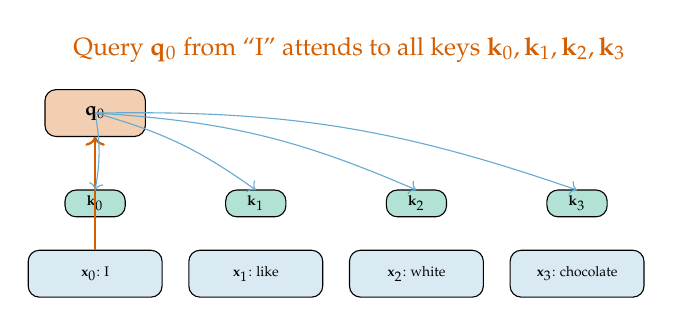
\begin{tikzpicture}[scale=0.85, every node/.style={font=\scriptsize}]
    \foreach \i/\w in {0/I, 1/like, 2/white, 3/chocolate} {
        \pgfmathsetmacro\x{\i*2.4}
        \draw[fill=blue!15, rounded corners] (\x, 0) rectangle (\x+2.0, 0.7);
        \node[font=\tiny] at (\x+1.0, 0.35) {$\vx_\i$: \w};
    }

    \foreach \i in {0,...,3} {
        \pgfmathsetmacro\x{\i*2.4}
        \draw[fill=green!30, rounded corners] (\x+0.55, 1.2) rectangle (\x+1.45, 1.6);
        \node[font=\tiny] at (\x+1.0, 1.4) {$\vk_\i$};
    }

    \draw[fill=red!30, rounded corners] (0.25, 2.4) rectangle (1.75, 3.1);
    \node at (1.0, 2.75) {$\vq_0$};
    \draw[->, red, thick] (1.0, 0.7) -- (1.0, 2.4);

    \foreach \i in {0,...,3} {
        \pgfmathsetmacro\x{\i*2.4}
        \draw[->, blue!60] (1.0, 2.75) to[bend left=10] (\x+1.0, 1.6);
    }

    \node[font=\small, red] at (4.8, 3.7) {Query $\vq_0$ from ``I'' attends to all keys $\vk_0, \vk_1, \vk_2, \vk_3$};
\end{tikzpicture}
\end{center}

\vspace{6pt}
\textbf{For position 0 (``I''):}
\begin{itemize}
    \item Project: $\vq_0 = \vW_Q \vx_0$, $\vk_j = \vW_K \vx_j$, $\vv_j = \vW_V \vx_j$ for all $j$.
    \item Score: $e_{0,j} = \vq_0^\top \vk_j / \sqrt{d_k}$.
    \item Weights: $\alpha_{0,j} = \softmax_j(e_{0,j})$.
    \item Output: $\vo_0 = \sum_j \alpha_{0,j} \vv_j$.
\end{itemize}
\end{frame}

\begin{frame}
\frametitle{Build-up: Every Position Attends to Every Other}

\textbf{Repeat the same procedure for $\vq_1, \vq_2, \vq_3$.}

\vspace{4pt}
\begin{center}
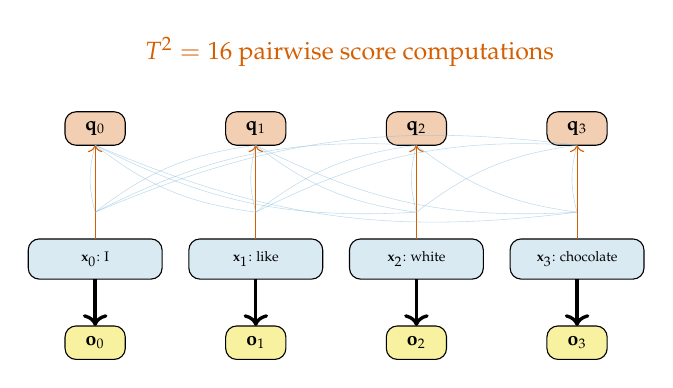
\begin{tikzpicture}[scale=0.85, every node/.style={font=\scriptsize}]
    \foreach \i/\w in {0/I, 1/like, 2/white, 3/chocolate} {
        \pgfmathsetmacro\x{\i*2.4}
        \draw[fill=blue!15, rounded corners] (\x, 0) rectangle (\x+2.0, 0.6);
        \node[font=\tiny] at (\x+1.0, 0.3) {$\vx_\i$: \w};
    }

    \foreach \i in {0,...,3} {
        \pgfmathsetmacro\x{\i*2.4}
        \draw[fill=red!30, rounded corners] (\x+0.55, 2) rectangle (\x+1.45, 2.5);
        \node at (\x+1.0, 2.25) {$\vq_\i$};
        \draw[->, red, thin] (\x+1.0, 0.6) -- (\x+1.0, 2);
    }

    \foreach \i in {0,...,3} {
        \foreach \j in {0,...,3} {
            \pgfmathsetmacro\sx{\i*2.4+1.0}
            \pgfmathsetmacro\dx{\j*2.4+1.0}
            \draw[blue!50, very thin, opacity=0.5] (\sx, 2) to[bend right=15] (\dx, 1);
        }
    }
    \node[font=\small, red] at (4.8, 3.4) {$T^2 = 16$ pairwise score computations};

    \foreach \i in {0,...,3} {
        \pgfmathsetmacro\x{\i*2.4}
        \draw[fill=yellow!50, rounded corners] (\x+0.55, -1.2) rectangle (\x+1.45, -0.7);
        \node at (\x+1.0, -0.95) {$\vo_\i$};
        \draw[->, very thick] (\x+1.0, 0) -- (\x+1.0, -0.7);
    }
\end{tikzpicture}
\end{center}

\vspace{4pt}
\textbf{In matrix form,} all of this is just one operation:
\[
    \vO = \softmax\!\left(\frac{\vQ \vK^\top}{\sqrt{d_k}}\right) \vV.
\]

\textcolor{red}{The whole sentence is processed \textbf{in parallel}, not sequentially like an RNN.}
\end{frame}

\begin{frame}
\frametitle{Self-Attention as a Matrix}

\textbf{The attention matrix has one row per query and one column per key.}

\vspace{6pt}
\begin{center}
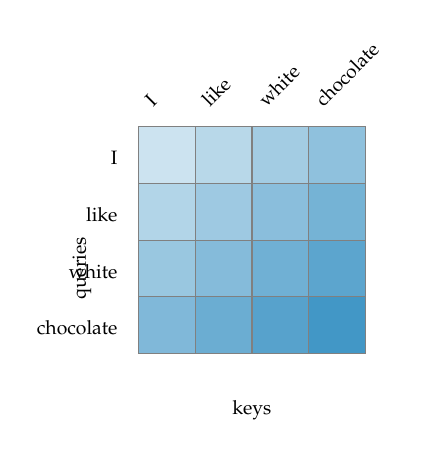
\begin{tikzpicture}[scale=0.72, every node/.style={font=\scriptsize}]
    \foreach \i/\w in {0/I, 1/like, 2/white, 3/chocolate} {
        \node[rotate=45, anchor=west] at (\i+1.05, 0.3) {\w};
        \node[anchor=east] at (0.8, -\i-0.55) {\w};
    }
    \foreach \i in {0,...,3} {
        \foreach \j in {0,...,3} {
            \pgfmathtruncatemacro\shade{20 + 10*\i + 8*\j}
            \fill[blue!\shade] (\j+1, -\i-1) rectangle (\j+2, -\i);
            \draw[gray, thin] (\j+1, -\i-1) rectangle (\j+2, -\i);
        }
    }
    \node at (3, -5.0) {keys};
    \node[rotate=90] at (0.0, -2.5) {queries};
\end{tikzpicture}
\end{center}

\vspace{4pt}
Row $i$ is a probability distribution: which tokens should position $i$ read from?
\end{frame}

\begin{frame}
\frametitle{Self-Attention vs CNN vs RNN}

\textbf{Receptive field comparison.} How does each layer connect position $i$ to position $j$?

\vspace{4pt}
\begin{center}
\renewcommand{\arraystretch}{1.18}
\scriptsize
\begin{tabular}{l c c c}
\toprule
\textbf{Property} & \textbf{RNN} & \textbf{CNN} & \textbf{Self-attention} \\
\midrule
Path length, $i \to j$ & $O(|i - j|)$ & $O(\log_k T)$ & $O(1)$ \\
Parallelism & sequential & parallel & parallel \\
Receptive field per layer & 1 step & kernel size & full sequence \\
Inductive bias & order & locality & permutation-equivariant \\
\bottomrule
\end{tabular}
\end{center}

\vspace{5pt}
\textbf{What the table says:}
\begin{itemize}
    \item RNN needs $|i - j|$ steps to connect distant positions.
    \item CNN needs $\log$ depth (with dilated convs).
    \item Self-attention connects all positions in one step, but needs positional encoding for order.
\end{itemize}

\vspace{4pt}
\textcolor{red}{Self-attention trades inductive bias for flexibility.}
\end{frame}

\begin{frame}
\frametitle{Computational Complexity}

\textbf{Per-layer cost} for a sequence of length $T$ and embedding dim $D$:

\vspace{4pt}
\begin{center}
\renewcommand{\arraystretch}{1.15}
\scriptsize
\begin{tabular}{l c c}
\toprule
\textbf{Layer type} & \textbf{Compute} & \textbf{Comment} \\
\midrule
RNN & $O(T \cdot D^2)$ & dominated by recurrent matmul \\
CNN (kernel $k$) & $O(k \cdot T \cdot D^2)$ & still linear in $T$ \\
Self-attention & $O(T^2 \cdot D)$ & quadratic in $T$ \\
\bottomrule
\end{tabular}
\end{center}

\vspace{5pt}
\textbf{Crossover.} Self-attention is cheaper than RNN when $T < D$ (typical for sentences with $T \approx 50$, $D \approx 512$).

\vspace{5pt}
\textbf{For very long sequences} ($T \gg D$, e.g.\ entire documents): self-attention becomes expensive. This motivates:
\begin{itemize}
    \item Sparse attention (Longformer, BigBird).
    \item Linear attention (Performer, Linformer).
    \item Flash attention (efficient implementation).
\end{itemize}

\textcolor{blue}{For typical NLP tasks, $T^2$ lets every word talk to every other.}
\end{frame}

\begin{frame}
\frametitle{Section Summary}

\textbf{Self-attention in one slide:}

\vspace{6pt}
\begin{enumerate}
    \item Take an input sequence $\vX \in \R^{T \times D}$.
    \item Project three ways: $\vQ = \vX \vW_Q^\top$, $\vK = \vX \vW_K^\top$, $\vV = \vX \vW_V^\top$.
    \item Compute pairwise scores: $\vQ \vK^\top \in \R^{T \times T}$.
    \item Normalize: $\softmax(\vQ \vK^\top / \sqrt{d_k})$.
    \item Aggregate: multiply by $\vV$.
\end{enumerate}

\vspace{8pt}
\textbf{Properties:}
\begin{itemize}
    \item Every position connects to every other in one step ($O(1)$ path length).
    \item Fully parallel.
    \item No notion of order (yet -- Lecture 9 fixes this with positional encoding).
\end{itemize}

\vspace{6pt}
\textcolor{red}{Coming up:} we still owe an explanation of the $\sqrt{d_k}$ scaling. It's not cosmetic.
\end{frame}


% ============================================================
\section{Why \texorpdfstring{$\sqrt{d_k}$}{sqrt(d\_k)}?}
% ============================================================

\begin{transitionframe}
\begin{center}
{\Huge \textbf{Why $\sqrt{d_k}$?}}\\[10pt]
{\large The Central Limit Theorem in action}
\end{center}
\end{transitionframe}

\begin{frame}
\frametitle{The Softmax Saturation Problem}

\textbf{Reminder.} Softmax with input scale matters a lot:

\vspace{6pt}
\begin{center}
\renewcommand{\arraystretch}{1.3}
\small
\begin{tabular}{c c c}
\toprule
\textbf{Logits} & \textbf{Softmax} & \textbf{Comment} \\
\midrule
$(1, 0, 0)$ & $(0.58, 0.21, 0.21)$ & gentle, gradients flow \\
$(5, 0, 0)$ & $(0.99, 0.007, 0.007)$ & sharper \\
$(20, 0, 0)$ & $(\approx 1, 10^{-9}, 10^{-9})$ & saturated, gradients vanish \\
\bottomrule
\end{tabular}
\end{center}

\vspace{10pt}
\textbf{Why gradients vanish at saturation.} The softmax Jacobian has entries
\[
    \frac{\partial \softmax(\vz)_i}{\partial z_j} = \softmax(\vz)_i \cdot (\delta_{ij} - \softmax(\vz)_j).
\]

When one entry is $\approx 1$ and the rest are $\approx 0$, every derivative is $\approx 0$.

\vspace{6pt}
\textcolor{red}{We need to make sure the inputs to softmax stay at a reasonable scale -- typically $O(1)$.}
\end{frame}

\begin{frame}
\frametitle{Setup: What Are the Dot-Product Scores?}

\textbf{Assumption} (reasonable at initialization): entries of $\vq$ and $\vk$ are i.i.d. with mean 0 and variance 1.
\[
    q_i \sim \mathcal{N}(0, 1), \qquad k_i \sim \mathcal{N}(0, 1), \qquad q_i \perp k_j.
\]

\vspace{8pt}
\textbf{Dot product:}
\[
    s = \vq^\top \vk = \sum_{i=1}^{d_k} q_i k_i.
\]

\vspace{8pt}
\textbf{Goal.} Compute the distribution of $s$.

\vspace{6pt}
\textbf{Why this matters.} The score $s$ feeds directly into softmax. If $s$ has wide spread, softmax saturates.
\end{frame}

\begin{frame}
\frametitle{CLT Derivation: One Term}

\textbf{Step 1: Mean of each term.}
\[
    \E[q_i k_i] \;=\; \E[q_i] \cdot \E[k_i] \;=\; 0 \cdot 0 \;=\; 0.
\]
(Using independence.)

\vspace{6pt}
\textbf{Step 2: Variance of each term.}
\begin{align*}
    \Var(q_i k_i) &= \E[(q_i k_i)^2] - (\E[q_i k_i])^2 \\
                  &= \E[q_i^2]\,\E[k_i^2] - 0 \\
                  &= 1 \cdot 1 \;=\; 1.
\end{align*}
\end{frame}

\begin{frame}
\frametitle{CLT Derivation: Sum of Terms}

\textbf{Step 3: Variance of the sum.} Since the $d_k$ terms are independent,
\[
    \Var(s) \;=\; \sum_{i=1}^{d_k} \Var(q_i k_i) \;=\; d_k.
\]

\vspace{4pt}
\textbf{Step 4: Apply CLT.} For large $d_k$,
\[
    s \;\sim\; \mathcal{N}(0, d_k) \quad \text{approximately}.
\]
Standard deviation: $\sqrt{d_k}$.
\end{frame}

\begin{frame}
\frametitle{Why This Is Bad Without Scaling}

\textbf{Typical values} of $d_k$ in modern Transformers:
\begin{itemize}
    \item BERT-base: $d_k = 64$, so $\sqrt{d_k} = 8$.
    \item GPT-3 small heads: $d_k = 128$, so $\sqrt{d_k} \approx 11$.
    \item Large models: $d_k = 256$, so $\sqrt{d_k} = 16$.
\end{itemize}

\vspace{8pt}
\textbf{Consequence.} Scores typically range over $\pm 2 \sqrt{d_k}$, so $\pm 16$ for BERT-base.

\vspace{4pt}
Plugging into softmax: the largest logit dominates by a factor of $e^{16} \approx 9 \times 10^6$. Output is near one-hot. Gradients vanish.

\vspace{8pt}
\textbf{Empirical signature without scaling:} training stalls within the first hundreds of steps; loss plateaus at random.

\vspace{6pt}
\textcolor{red}{The fix is one line of code: divide by $\sqrt{d_k}$ before softmax.}
\end{frame}

\begin{frame}
\frametitle{The Fix: Divide by $\sqrt{d_k}$}

\textbf{Define the scaled score:}
\[
    \tilde{s} \;=\; \frac{s}{\sqrt{d_k}} \;=\; \frac{\vq^\top \vk}{\sqrt{d_k}}.
\]

\vspace{6pt}
\textbf{Variance of the scaled score:}
\[
    \Var(\tilde{s}) \;=\; \frac{\Var(s)}{d_k} \;=\; \frac{d_k}{d_k} \;=\; 1.
\]

\vspace{8pt}
\textbf{So:} $\tilde s \sim \mathcal{N}(0, 1)$ approximately. Softmax inputs stay at $O(1)$ scale, gradients flow.

\vspace{8pt}
\begin{tikzpicture}
\node [mybox] (box){%
    \begin{minipage}{0.93\textwidth}
    \vspace{-4pt}
    \begin{center}
    $\displaystyle \text{Attention}(\vQ, \vK, \vV) \;=\; \softmax\!\left(\frac{\vQ \vK^\top}{\sqrt{d_k}}\right) \vV$ \\[4pt]
    The $\sqrt{d_k}$ normalizer keeps softmax inputs at unit variance.
    \end{center}
    \end{minipage}
};
\node[fancytitle, right=10pt] at (box.north west) {Scaled dot-product attention};
\end{tikzpicture}

\note{HW3 note: this is the derivation used in Problem 3(a)ii.}
\end{frame}

\begin{frame}
\frametitle{Numerical Mini-Example: Why Scaling Helps}

\textbf{Use a common head dimension:} $d_k = 64$, so $\sqrt{d_k} = 8$.

\vspace{4pt}
\begin{center}
\renewcommand{\arraystretch}{1.2}
\small
\begin{tabular}{l c c}
\toprule
& \textbf{without scaling} & \textbf{with scaling} \\
\midrule
raw dot product & $16$ & $16$ \\
score into softmax & $16$ & $16/8 = 2$ \\
example logits & $(16,0,0)$ & $(2,0,0)$ \\
softmax output & $(\approx 1, 10^{-7}, 10^{-7})$ & $(0.79, 0.11, 0.11)$ \\
\bottomrule
\end{tabular}
\end{center}

\vspace{6pt}
\[
    \frac{\vq^\top \vk}{\sqrt{d_k}}
    =
    \frac{16}{8}
    =
    2.
\]

\textcolor{red}{Interpretation:} scaling prevents one key from winning too aggressively at initialization, so gradients remain useful.
\end{frame}


% ============================================================
\section{Multi-Head Attention}
% ============================================================

\begin{transitionframe}
\begin{center}
{\Huge \textbf{Multi-Head Attention}}\\[10pt]
{\large Many attention computations in parallel}
\end{center}
\end{transitionframe}

\begin{frame}
\frametitle{Why Multiple Heads?}

\textbf{One head learns one kind of attention pattern.}

\vspace{6pt}
\textbf{Examples of patterns that may emerge:}
\begin{itemize}
    \item Head A: attend to syntactic dependencies (subject $\leftrightarrow$ verb).
    \item Head B: attend to coreference (pronoun $\leftrightarrow$ antecedent).
    \item Head C: attend to nearby words (local structure).
    \item Head D: attend to entities mentioned earlier in the document.
\end{itemize}

\vspace{8pt}
\textbf{One single attention map cannot capture all of these.}

\vspace{8pt}
\textbf{Solution.} Run several attention computations in parallel -- one per ``head'' -- and combine the outputs.

\vspace{6pt}
\textcolor{red}{Multi-head attention $=$ ensemble of attention computations with different learned projections.}
\end{frame}

\begin{frame}
\frametitle{Multi-Head: The Math}

\textbf{Setup.} Number of heads $h$. Each head has its own projection matrices.

\vspace{4pt}
For head $i = 1, \ldots, h$:
\[
    \vQ^i = \vX \vW_Q^{i,\top}, \qquad \vK^i = \vX \vW_K^{i,\top}, \qquad \vV^i = \vX \vW_V^{i,\top}.
\]

\vspace{6pt}
\textbf{Per-head attention:}
\[
    \vO^i \;=\; \softmax\!\left(\frac{\vQ^i (\vK^i)^\top}{\sqrt{d_k}}\right) \vV^i \;\in\; \R^{T \times d_v}.
\]

\vspace{8pt}
\textbf{Concatenate the head outputs:}
\[
    \vO_\text{cat} \;=\; [\vO^1,\, \vO^2,\, \ldots,\, \vO^h] \;\in\; \R^{T \times h d_v}.
\]

\vspace{6pt}
\textbf{Final output projection by $\vW_O \in \R^{D \times h d_v}$:}
\[
    \vO \;=\; \vO_\text{cat}\, \vW_O^\top \;\in\; \R^{T \times D}.
\]

\vfill
{\scriptsize\textcolor{blue}{HW3 note: track the concat-then-$\vW_O$ step carefully.}}
\end{frame}

\begin{frame}
\frametitle{Multi-Head: Shape Cheat-Sheet}

\textbf{All shapes in one place:}

\vspace{4pt}
\begin{center}
\renewcommand{\arraystretch}{1.18}
\scriptsize
\begin{tabular}{l l l}
\toprule
\textbf{Tensor} & \textbf{Shape} & \textbf{Description} \\
\midrule
$\vX$ & $T \times D$ & input sequence \\
$\vW_Q^i,\, \vW_K^i$ & $d_k \times D$ & per-head Q/K projections \\
$\vW_V^i$ & $d_v \times D$ & per-head V projection \\
$\vQ^i,\, \vK^i$ & $T \times d_k$ & per-head queries/keys \\
$\vV^i$ & $T \times d_v$ & per-head values \\
$\vO^i$ & $T \times d_v$ & per-head output \\
$\vO_\text{cat}$ & $T \times h d_v$ & concatenated heads \\
$\vW_O$ & $D \times h d_v$ & output projection \\
$\vO$ & $T \times D$ & final output \\
\bottomrule
\end{tabular}
\end{center}

\vspace{4pt}
\textbf{Common choice:} $d_k = d_v = D / h$, so the per-head dim is small and the total parameter count matches a single-head attention with dim $D$.

\vspace{2pt}
\textcolor{red}{E.g., BERT-base: $D = 768$, $h = 12$, so $d_k = d_v = 64$.}
\end{frame}

\begin{frame}
\frametitle{Multi-Head: Visual}

\begin{center}
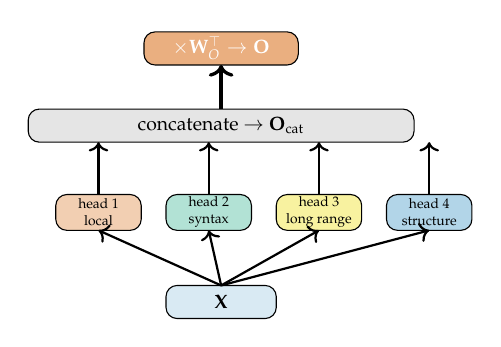
\begin{tikzpicture}[scale=0.7, every node/.style={font=\scriptsize}]
    \draw[fill=blue!15, rounded corners] (-1, 0) rectangle (1, 0.6);
    \node at (0, 0.3) {$\vX$};

    \foreach \i/\name/\col in {1/local/red!30, 2/syntax/green!30, 3/long range/yellow!50, 4/structure/blue!30} {
        \pgfmathsetmacro\x{\i*2 - 5}
        \draw[fill=\col, rounded corners] (\x, 1.6) rectangle (\x+1.55, 2.25);
        \node[align=center, font=\tiny] at (\x+0.775, 1.93) {head \i\\\name};
        \draw[->, thick] (0, 0.6) -- (\x+0.775, 1.6);
    }

    \draw[fill=gray!20, rounded corners] (-3.5, 3.2) rectangle (3.5, 3.8);
    \node at (0, 3.5) {concatenate $\to$ $\vO_\text{cat}$};
    \foreach \i in {1,...,4} {
        \pgfmathsetmacro\x{\i*2 - 5}
        \draw[->, thick] (\x+0.775, 2.25) -- (\x+0.775, 3.2);
    }

    \draw[fill=red!50, rounded corners] (-1.4, 4.6) rectangle (1.4, 5.2);
    \node[white, font=\scriptsize] at (0, 4.9) {$\times \vW_O^\top \to \vO$};
    \draw[->, very thick] (0, 3.8) -- (0, 4.6);
\end{tikzpicture}
\end{center}

\vspace{4pt}
\textbf{Reading the diagram:}
\begin{itemize}
    \item Same input $\vX$ feeds all $h$ heads (here $h = 4$).
    \item Each head can learn a different relation because it has its own $\vW_Q^i, \vW_K^i, \vW_V^i$.
    \item Outputs are concatenated and projected by a single $\vW_O$.
\end{itemize}
\end{frame}

\begin{frame}
\frametitle{Section Summary}

\textbf{Multi-head attention recipe:}

\vspace{6pt}
\begin{enumerate}
    \item Project $\vX$ into $h$ different (Q, K, V) triplets, one per head.
    \item Run scaled dot-product attention independently in each head.
    \item Concatenate the $h$ outputs.
    \item Project back to dim $D$ via $\vW_O$.
\end{enumerate}

\vspace{8pt}
\textbf{What multi-head buys you:}
\begin{itemize}
    \item Each head can specialize on a different attention pattern.
    \item Same total compute as single-head with full dim (when $d_k = D/h$).
    \item Empirically much better than single-head.
\end{itemize}

\vspace{6pt}
\textcolor{red}{Coming up:} how do you actually implement this in PyTorch? And what about masks?
\end{frame}


% ============================================================
\section{Practical Implementation}
% ============================================================

\begin{transitionframe}
\begin{center}
{\Huge \textbf{Practical Implementation}}\\[10pt]
{\large Shapes, masks, PyTorch}
\end{center}
\end{transitionframe}

\begin{frame}[fragile]
\frametitle{PyTorch: nn.MultiheadAttention}

\textbf{Built-in module:} \texttt{torch.nn.MultiheadAttention}.

\vspace{4pt}
\begin{lstlisting}
import torch.nn as nn

mha = nn.MultiheadAttention(
    embed_dim=768,    # = D
    num_heads=12,     # = h, so d_k = d_v = 64
    batch_first=True  # use (batch, T, D) shape
)

# x: (batch=32, T=50, D=768)
out, attn_weights = mha(x, x, x)   # self-attention: Q=K=V=x
\end{lstlisting}

\vspace{6pt}
\textbf{Shapes returned:}
\begin{itemize}
    \item \texttt{out}: \texttt{(32, 50, 768)} -- same shape as input.
    \item \texttt{attn\_weights}: \texttt{(32, 50, 50)} -- attention map per batch element.
\end{itemize}

\vspace{6pt}
\textbf{For cross-attention:} \texttt{mha(query, key\_value, key\_value)}.

\vspace{4pt}
\textcolor{blue}{The module hides the projection matrices and the concat-then-W\_O step.}
\end{frame}

\begin{frame}
\frametitle{Causal Mask (for Language Models)}

\textbf{Problem.} A decoder predicting the next word must not see future tokens.

\vspace{6pt}
\textbf{Fix.} Add a \textbf{causal mask} to the score matrix \emph{before} softmax:
\[
    e_{i,j} \;=\;
    \begin{cases}
        \vq_i^\top \vk_j / \sqrt{d_k}, & j \leq i \\
        -\infty, & j > i.
    \end{cases}
\]

\vspace{3pt}
After softmax, the $-\infty$ entries become 0.

\vspace{3pt}
\begin{center}
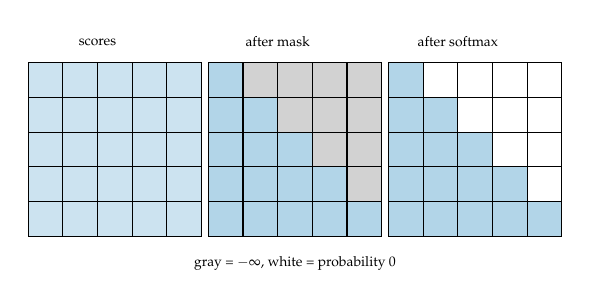
\begin{tikzpicture}[scale=0.44, every node/.style={font=\tiny}]
    \node at (2, 0.6) {scores};
    \node at (7.2, 0.6) {after mask};
    \node at (12.4, 0.6) {after softmax};
    \foreach \offset/\mode in {0/0, 5.2/1, 10.4/2} {
        \foreach \i in {0,...,4} {
            \foreach \j in {0,...,4} {
                \ifnum\mode=0
                    \fill[blue!20] (\offset+\j, -\i) rectangle (\offset+\j+1, -\i-1);
                \else
                    \ifnum\j>\i
                        \ifnum\mode=1 \fill[gray!35] (\offset+\j, -\i) rectangle (\offset+\j+1, -\i-1);
                        \else \fill[white] (\offset+\j, -\i) rectangle (\offset+\j+1, -\i-1);
                        \fi
                    \else
                        \fill[blue!30] (\offset+\j, -\i) rectangle (\offset+\j+1, -\i-1);
                    \fi
                \fi
                \draw[thin] (\offset+\j, -\i) rectangle (\offset+\j+1, -\i-1);
            }
        }
    }
    \node at (7.7, -5.8) {gray = $-\infty$, white = probability 0};
\end{tikzpicture}
\end{center}

\textcolor{red}{Position $i$ can only attend to positions $\leq i$.}
\end{frame}

\begin{frame}
\frametitle{Numerical Mini-Example: Causal Mask}

\textbf{Suppose position $i=3$ scores five keys. Key 4 is in the future.}

\vspace{4pt}
\[
    \text{raw scores}
    =
    (1.2,\; 0.5,\; 2.0,\; 0.7,\; 3.1).
\]

\vspace{2pt}
\[
    \text{after causal mask}
    =
    (1.2,\; 0.5,\; 2.0,\; 0.7,\; -\infty).
\]

\vspace{2pt}
\begin{align*}
    \exp(1.2,0.5,2.0,0.7,-\infty)
    &\approx (3.32,\;1.65,\;7.39,\;2.01,\;0), \\
    \softmax
    &\approx (0.23,\;0.11,\;0.51,\;0.14,\;0).
\end{align*}

\textcolor{red}{Interpretation:} even if the future token had the largest raw score ($3.1$), the mask forces its probability to exactly zero.
\end{frame}

\begin{frame}[fragile]
\frametitle{Padding Mask (for Batched Sequences)}

\textbf{Problem.} Batches contain sequences of different lengths, padded to the longest. We shouldn't attend to padding tokens.

\vspace{6pt}
\textbf{Example batch:}
\begin{itemize}
    \item Sequence 1: ``the cat sat'' (length 3)
    \item Sequence 2: ``hello'' (length 1)
    \item Padded to length 5: \texttt{[the, cat, sat, PAD, PAD]} and \texttt{[hello, PAD, PAD, PAD, PAD]}.
\end{itemize}

\vspace{8pt}
\textbf{Fix.} Mask out the padding positions in keys (so no query attends to them):
\[
    e_{i,j} \;=\; -\infty \quad \text{if $j$ is a padding position}.
\]

\vspace{6pt}
\textbf{In PyTorch:}
\begin{lstlisting}[basicstyle=\ttfamily\scriptsize]
key_padding_mask = (input_ids == PAD_TOKEN)   # (batch, T) of bools
out, _ = mha(x, x, x, key_padding_mask=key_padding_mask)
\end{lstlisting}

\vspace{4pt}
\textcolor{blue}{Both masks (causal + padding) are commonly combined in language models.}
\end{frame}


% ============================================================
\section{Econ Applications and Bridge to Transformers}
% ============================================================

\begin{transitionframe}
\begin{center}
{\Huge \textbf{Econ Applications \& Bridge to Lecture 9}}
\end{center}
\end{transitionframe}

\begin{frame}
\frametitle{Attention for Time-Series Forecasting}

\textbf{Temporal Fusion Transformer} (Lim et al., \emph{IJF} 2021).

\vspace{6pt}
\textbf{Architecture for forecasting macro time series:}
\begin{itemize}
    \item Embed each observation (numerical + categorical features).
    \item LSTM for short-range temporal patterns.
    \item Self-attention over the full history for long-range dependencies.
    \item Quantile loss for uncertainty estimates.
\end{itemize}

\vspace{8pt}
\textbf{Why attention helps for macro forecasting:}
\begin{itemize}
    \item Past crises (e.g., 2008, 2020) are sparse, distant events.
    \item RNNs struggle to remember them; attention can directly reference them.
    \item Diagnostics: attention weights can highlight \emph{which past periods the model uses}.
\end{itemize}

\vspace{6pt}
\textcolor{red}{For econ: attention weights can be useful diagnostics, though not complete explanations.}
\end{frame}

\begin{frame}
\frametitle{Attention for Tabular Data}

\textbf{TabNet} (Arik \& Pfister, AAAI 2021) and \textbf{FT-Transformer} (Gorishniy et al., NeurIPS 2021).

\vspace{6pt}
\textbf{Setup.} Each row of a tabular dataset has features $(x_1, x_2, \ldots, x_F)$ -- e.g., a credit application.

\vspace{6pt}
\textbf{The trick.} Embed each \emph{feature} as a vector, then run self-attention over the feature embeddings.

\vspace{4pt}
The model learns which features matter for the prediction \emph{conditionally on other features}.

\vspace{8pt}
\textbf{Applied econ use cases:}
\begin{itemize}
    \item Default prediction with attention weights as interpretability.
    \item Demand forecasting with feature attention.
    \item Heterogeneous treatment effect estimation: which covariates moderate the treatment?
\end{itemize}

\vspace{6pt}
\textcolor{blue}{Caveat:} for small-to-medium tabular data, gradient boosting (XGBoost, LightGBM) often still wins. Attention shines when you have $> 10^4$ rows and rich categorical features.
\end{frame}

\begin{frame}
\frametitle{Attention for Text-as-Data in Econ}

\textbf{Modern econ NLP pipelines use Transformer encoders} (BERT, RoBERTa, BETO for Spanish).

\vspace{8pt}
\textbf{Typical workflow:}
\begin{enumerate}
    \item Take a corpus (FOMC minutes, central bank speeches, news, earnings calls).
    \item Tokenize and feed through a pretrained Transformer.
    \item Extract the contextual embeddings (one vector per token, or one per document).
    \item Use those as features for downstream econ analysis.
\end{enumerate}

\vspace{8pt}
\textbf{Recent papers:}
\begin{itemize}
    \item Hansen, Kazinnik (2023): Fed sentiment from FOMC text via BERT embeddings.
    \item Bybee, Kelly, Manela, Xiu (2024, JFE): news topic attention for asset prices.
    \item Ash et al. (2024): judicial reasoning from opinions.
\end{itemize}

\vspace{6pt}
\textcolor{red}{These all rely on attention's ability to produce context-dependent embeddings -- the topic that's been our through-line.}
\end{frame}

\begin{frame}
\frametitle{What's Missing: Bridge to Lecture 9}

\textbf{We've built scaled dot-product self-attention.} What's left to assemble a Transformer?

\vspace{6pt}
\begin{enumerate}
    \item \textbf{Positional encoding.} Self-attention is permutation-equivariant -- it has no notion of word order. We need to inject position information.

    \vspace{4pt}
    \item \textbf{Layer normalization.} Normalize each token's vector to stabilize training.

    \vspace{4pt}
    \item \textbf{Residual connections.} $\vO = \text{Attention}(\vX) + \vX$. Helps gradient flow.

    \vspace{4pt}
    \item \textbf{Feed-forward sublayer.} A position-wise MLP after attention -- adds capacity.

    \vspace{4pt}
    \item \textbf{Stack many blocks.} GPT, BERT, T5 are all just stacks of these blocks.
\end{enumerate}

\vspace{8pt}
\textcolor{red}{Lecture 9} puts the pieces together: \textit{Attention Is All You Need} (Vaswani et al.\ 2017) and the modern Transformer architecture.
\end{frame}


% ============================================================
\section{Summary and Next Steps}
% ============================================================

\begin{transitionframe}
\begin{center}
{\Huge \textbf{Summary \& Next Steps}}
\end{center}
\end{transitionframe}

\begin{frame}
\frametitle{One Mechanism, Many Settings}

\textbf{The same attention recipe appeared all lecture:}

\vspace{10pt}
\begin{center}
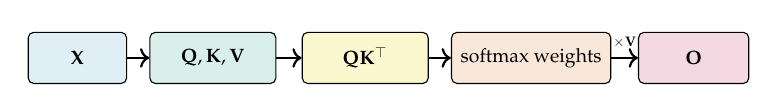
\begin{tikzpicture}[scale=0.86, every node/.style={font=\scriptsize}]
    \node[draw, fill=blue!12, rounded corners=2pt, minimum width=1.25cm, minimum height=0.65cm] (x) at (0,0) {$\vX$};
    \node[draw, fill=green!15, rounded corners=2pt, minimum width=1.6cm, minimum height=0.65cm] (qkv) at (2,0) {$\vQ,\vK,\vV$};
    \node[draw, fill=yellow!25, rounded corners=2pt, minimum width=1.6cm, minimum height=0.65cm] (scores) at (4.25,0) {$\vQ\vK^\top$};
    \node[draw, fill=red!15, rounded corners=2pt, minimum width=1.8cm, minimum height=0.65cm] (weights) at (6.7,0) {softmax weights};
    \node[draw, fill=purple!15, rounded corners=2pt, minimum width=1.4cm, minimum height=0.65cm] (out) at (9.1,0) {$\vO$};

    \draw[->, thick] (x) -- (qkv);
    \draw[->, thick] (qkv) -- (scores);
    \draw[->, thick] (scores) -- (weights);
    \draw[->, thick] (weights) -- node[above, font=\tiny] {$\times \vV$} (out);
\end{tikzpicture}
\end{center}

\vspace{10pt}
\begin{itemize}
    \item \textbf{Bahdanau attention:} decoder state queries encoder states.
    \item \textbf{Self-attention:} each token queries every token in the same sequence.
    \item \textbf{Multi-head attention:} repeat this in parallel with different projections.
\end{itemize}
\end{frame}

\begin{frame}
\frametitle{Today's Big Ideas}

\begin{enumerate}
    \item \textbf{Bahdanau attention} solves the seq2seq bottleneck: let the decoder look at all encoder states with learned weights.

    \vspace{4pt}
    \item \textbf{Query-Key-Value} is the general abstraction. Q asks, K advertises, V contributes.

    \vspace{4pt}
    \item \textbf{Self-attention} reuses the same input for Q, K, V. It connects any two positions in one step.

    \vspace{4pt}
    \item \textbf{Scaled dot product.} The $\sqrt{d_k}$ factor keeps softmax inputs at unit variance (CLT argument).

    \vspace{4pt}
    \item \textbf{Multi-head attention} runs $h$ attention computations in parallel and projects back through $\vW_O$.

    \vspace{4pt}
    \item \textbf{Complexity tradeoff.} Self-attention is $O(T^2 D)$ vs RNN's $O(T D^2)$. Crossover at $T \approx D$.

    \vspace{4pt}
    \item \textbf{For econ:} attention gives interpretable, context-aware representations of text, time series, and tabular data.
\end{enumerate}
\end{frame}

\begin{frame}
\frametitle{Practical Recipes}

\textbf{When to use attention:}
\begin{itemize}
    \item Sequence length $T < D$: faster than RNN.
    \item Need to model long-range dependencies: better than RNN.
    \item Need interpretability via attention maps: clear win.
\end{itemize}

\vspace{6pt}
\textbf{When to be careful:}
\begin{itemize}
    \item Very long sequences ($T > 10{,}000$): consider sparse / linear attention.
    \item Small training data: attention may underperform LSTMs or boosted trees.
    \item Time series with strong autoregressive structure: hybrid models often win.
\end{itemize}

\vspace{8pt}
\textbf{Common pitfalls:}
\begin{itemize}
    \item Forgetting the $\sqrt{d_k}$ scaling -- training will stall.
    \item Forgetting padding mask -- the model attends to noise.
    \item Forgetting causal mask in a language model -- it cheats and looks at future tokens.
\end{itemize}
\end{frame}

\begin{frame}
\frametitle{Next Lecture: Transformers}

\textbf{Lecture 9:}
\begin{itemize}
    \item Positional encoding (sinusoidal and learned).
    \item Layer normalization and residual connections.
    \item The Transformer encoder and decoder blocks.
    \item \emph{Attention Is All You Need} (Vaswani et al.\ 2017).
    \item BERT vs GPT: encoder-only vs decoder-only.
    \item Tokenization: byte-pair encoding.
    \item Pretraining and fine-tuning.
\end{itemize}

\vspace{8pt}
\textbf{The big picture:}
\begin{center}
\textit{Embeddings $\to$ Attention $\to$ Self-attention $\to$ Transformer $\to$ LLMs}
\end{center}

\vspace{12pt}
\begin{center}
\Large \textcolor{blue}{\textbf{Questions?}}
\end{center}
\end{frame}

\begin{frame}
\frametitle{References}

\footnotesize
\begin{itemize}
    \item Bahdanau, D., Cho, K., \& Bengio, Y. (2014). Neural machine translation by jointly learning to align and translate. \textit{ICLR}.
    \item Sutskever, I., Vinyals, O., \& Le, Q. (2014). Sequence to sequence learning with neural networks. \textit{NeurIPS}.
    \item Vaswani, A., et al. (2017). Attention is all you need. \textit{NeurIPS}.
    \item Lim, B., Arik, S., Loeff, N., \& Pfister, T. (2021). Temporal fusion transformers for interpretable multi-horizon time series forecasting. \textit{IJF}.
    \item Arik, S., \& Pfister, T. (2021). TabNet: attentive interpretable tabular learning. \textit{AAAI}.
    \item Gorishniy, Y., et al. (2021). Revisiting deep learning models for tabular data. \textit{NeurIPS}.
    \item Devlin, J., Chang, M., Lee, K., \& Toutanova, K. (2019). BERT: pre-training of deep bidirectional transformers. \textit{NAACL}.
    \item Hansen, S., \& Kazinnik, S. (2023). Can ChatGPT decipher Fedspeak? \textit{Working paper}.
    \item Bybee, L., Kelly, B., Manela, A., \& Xiu, D. (2024). Business news and business cycles. \textit{Journal of Finance}.
\end{itemize}
\end{frame}


\end{document}
